\section{Road network of Dublin}

\subsection{OpenStreetMaps + JOSM}\label{ssec:netconvert}
\ac{OSM} is a free world map editor. It is community driven and features up-to-date geospatial information. For this reason, \ac{OSM} is chosen for this dissertation. Maps can be extracted straight from the website. A bounding box is used to extract the region of interest, and multiple APIs are available to download the necessary information within the bounding box. Since the data within a bounding box of a large urban area can be substantial, custom queries can also be made to omit unnecessary data. An example of this is to omit pedestrian walkways, storefront data and recreational areas from the map download query. 

\ac{JOSM} is an \ac{OSM} map editor. It is a tool for editing \ac{OSM} maps locally, and is used to contribute to the update of an \ac{OSM} map. \ac{JOSM} is useful in relation to this dissertation as there are some minor roads leading to parking lots that are not defined within an \ac{OSM} map. An example of this is the entrance to the Arnotts parking lot. \ac{JOSM} is used to add the alley leading to the entrance to the parking lot.

Another reason for choosing \ac{OSM} maps is that \ac{SUMO} directly supports \ac{OSM} map conversion for use within SUMO. NETCONVERT is a SUMO tool that translates an \ac{OSM} .xml map file to the supported \ac{SUMO} format \citep{SUMO2008NETCONVERT}. \ac{OSM} maps consists of ``ways" and ``nodes". ``Ways" represent each road within a map, and ``nodes" represent the junctions where ``ways" are connected.

Through NETCONVERT, a \ac{SUMO} readable map can be generated. The result can be seen in figure \ref{fig:SUMODUBLIN}.

\begin{figure}[h]
    \centering
    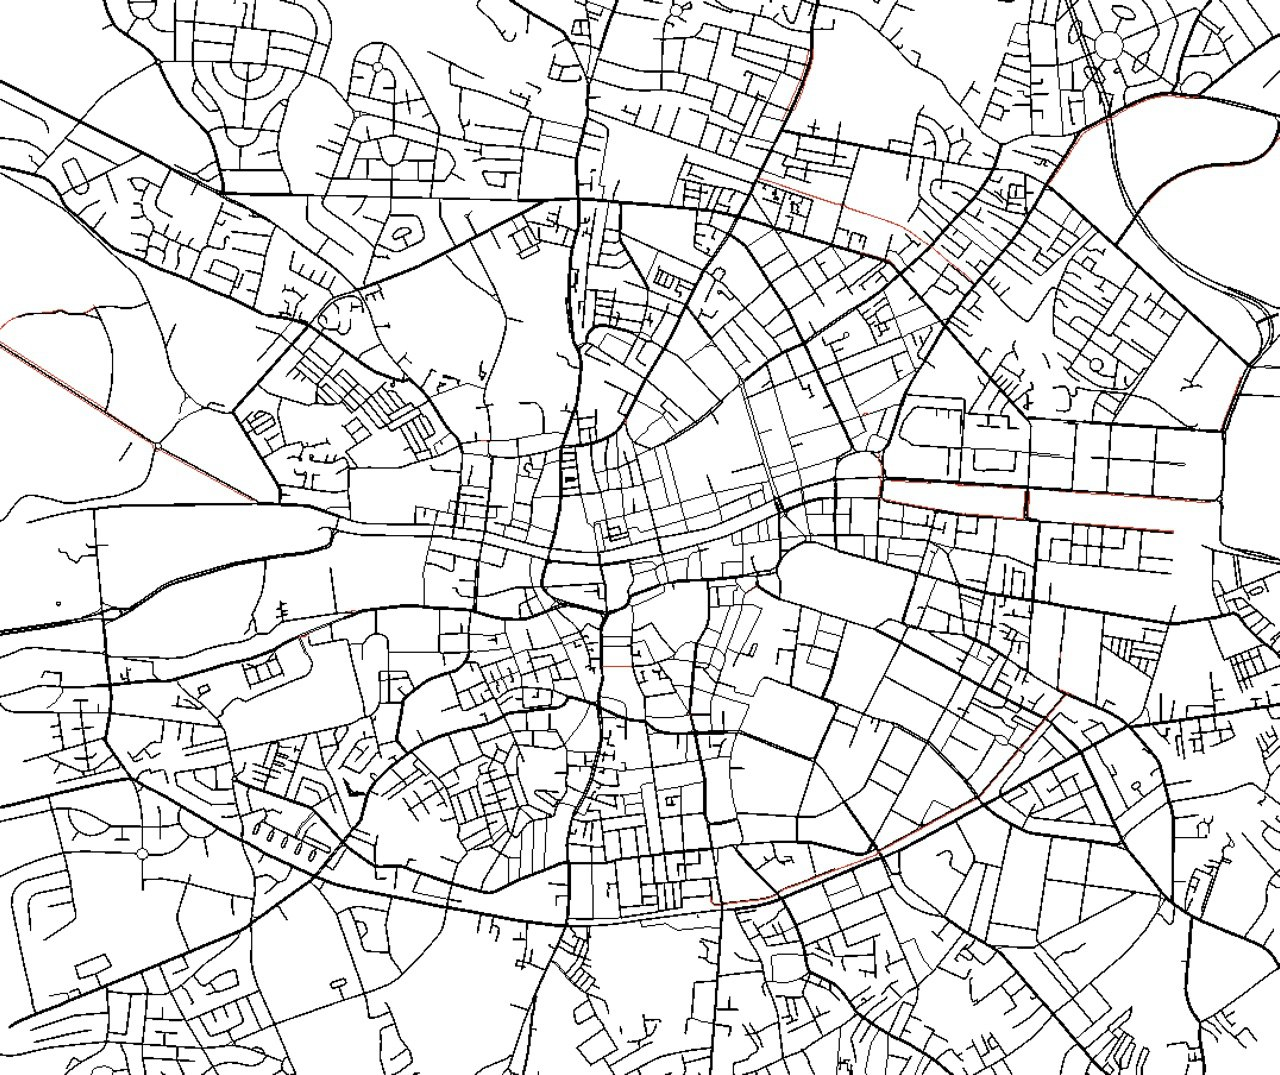
\includegraphics[width=\textwidth]{./Images/SUMODUBLIN.jpg}
    \caption{\ac{SUMO} Converted \ac{OSM} Map}
    \label{fig:SUMODUBLIN}
\end{figure}